
%%\documentclass[preprint,12pt]{elsarticle}

%% Use the option review to obtain double line spacing
\documentclass[preprint,review,12pt]{elsarticle}

%% Use the options 1p,twocolumn; 3p; 3p,twocolumn; 5p; or 5p,twocolumn
%% for a journal layout:
%% \documentclass[final,1p,times]{elsarticle}
%% \documentclass[final,1p,times,twocolumn]{elsarticle}
%% \documentclass[final,3p,times]{elsarticle}
%% \documentclass[final,3p,times,twocolumn]{elsarticle}
%% \documentclass[final,5p,times]{elsarticle}
%% \documentclass[final,5p,times,twocolumn]{elsarticle}

%% For including figures, graphicx.sty has been loaded in
%% elsarticle.cls. If you prefer to use the old commands
\usepackage{epsfig}
\usepackage[T1]{fontenc}
%% The amssymb package provides various useful mathematical symbols
\usepackage{amssymb}
%% The amsthm package provides extended theorem environments
%% \usepackage{amsthm}
%\usepackage[onehalfspacing]{setspace}
% Leave a blank line between paragraphs instead of using \\
%\usepackage{soul}
\usepackage{booktabs}   % For better table rules
\usepackage{siunitx}    % For alignment of numbers
\usepackage{adjustbox}  % To resize the table
%\usepackage{caption}    % For better caption formatting
\usepackage{subfig}
% For GitHub mark
\usepackage{graphicx}
%\usepackage{svg}

% Allow line-breaking of long urls and safe link handling
\PassOptionsToPackage{hyphens}{url} % improve url breaks
\usepackage[hidelinks]{hyperref}
\urlstyle{same}                     % keep the surrounding font for \url

% For numeric: compress and sort numbers like [1–3,5]
\biboptions{sort&compress}

% For author–year (if you compiled the class with ,authoryear):
% \biboptions{authoryear}


% For inline code
\usepackage{listings}

%% The lineno packages adds line numbers. Start line numbering with
%% \begin{linenumbers}, end it with \end{linenumbers}. Or switch it on
%% for the whole article with \linenumbers.
%% \usepackage{lineno}

\journal{Physica A}

\begin{document}

\begin{frontmatter}

%% Title, authors and addresses

%% use the tnoteref command within \title for footnotes;
%% use the tnotetext command for theassociated footnote;
%% use the fnref command within \author or \address for footnotes;
%% use the fntext command for theassociated footnote;
%% use the corref command within \author for corresponding author footnotes;
%% use the cortext command for theassociated footnote;
%% use the ead command for the email address,
%% and the form \ead[url] for the home page:
%% \title{Title\tnoteref{label1}}
%% \tnotetext[label1]{}
%% \author{Name\corref{cor1}\fnref{label2}}
%% \ead{email address}
%% \ead[url]{home page}
%% \fntext[label2]{}
%% \cortext[cor1]{}
%% \affiliation{organization={},
%%             addressline={},
%%             city={},
%%             postcode={},
%%             state={},
%%             country={}}
%% \fntext[label3]{}

\title{Spatial distribution of cancer stem cells promotes radioresistance in tumorspheres}



\author[famaf,ifeg]{Jerónimo Fotinós}
\author[famaf,ifeg]{Carlos A. Condat}
\author[ifeg]{Carlos S. Bederián}
\author[famaf,ifeg]{Lucas Barberis}

\affiliation[famaf]{organization={Facultad de Matemática, Astronomía, Física y Computación, Universidad Nacional de Córdoba},%Department and Organization
	addressline={Haya de la Torre s/n, Ciudad Universitaria}, 
	city={Córdoba},
	postcode={X5000HUA}, 
	state={Córdoba},
	country={Argentina}}

\affiliation[ifeg]{organization={Instituto de Física Enrique Gaviola, CONICET},%Department and Organization
	addressline={Haya de la Torre s/n, Ciudad Universitaria}, 
	city={Córdoba},
	postcode={X5000HUA}, 
	state={Córdoba},
	country={Argentina}}

\begin{abstract}
Cancer stem cells (CSCs) are particularly successful at fending off the effects of radiotherapy. Here we extend a computational model of tumorsphere growth, which allows us to track the location of the CSCs at all times, to show that their resistance at least partially stems from their preferential location near the spheroid center. Since radioresistance increases as oxygen availability decreases, and CSCs are found to be located predominantly away from the tumorsphere surface, these cells are especially well protected against radiation. Although this effect is minimal in early-stage tumorspheres, it becomes increasingly important as they grow. To further validate our hypothesis, we compare our results with those obtained by applying radiation to ersatz tumorspheres where the CSCs have been randomly redistributed, showing that this altered disposition substantially reduces their survival chances. These results are unchanged in the presence of necrosis.

\end{abstract}

%%Graphical abstract
\begin{graphicalabstract}
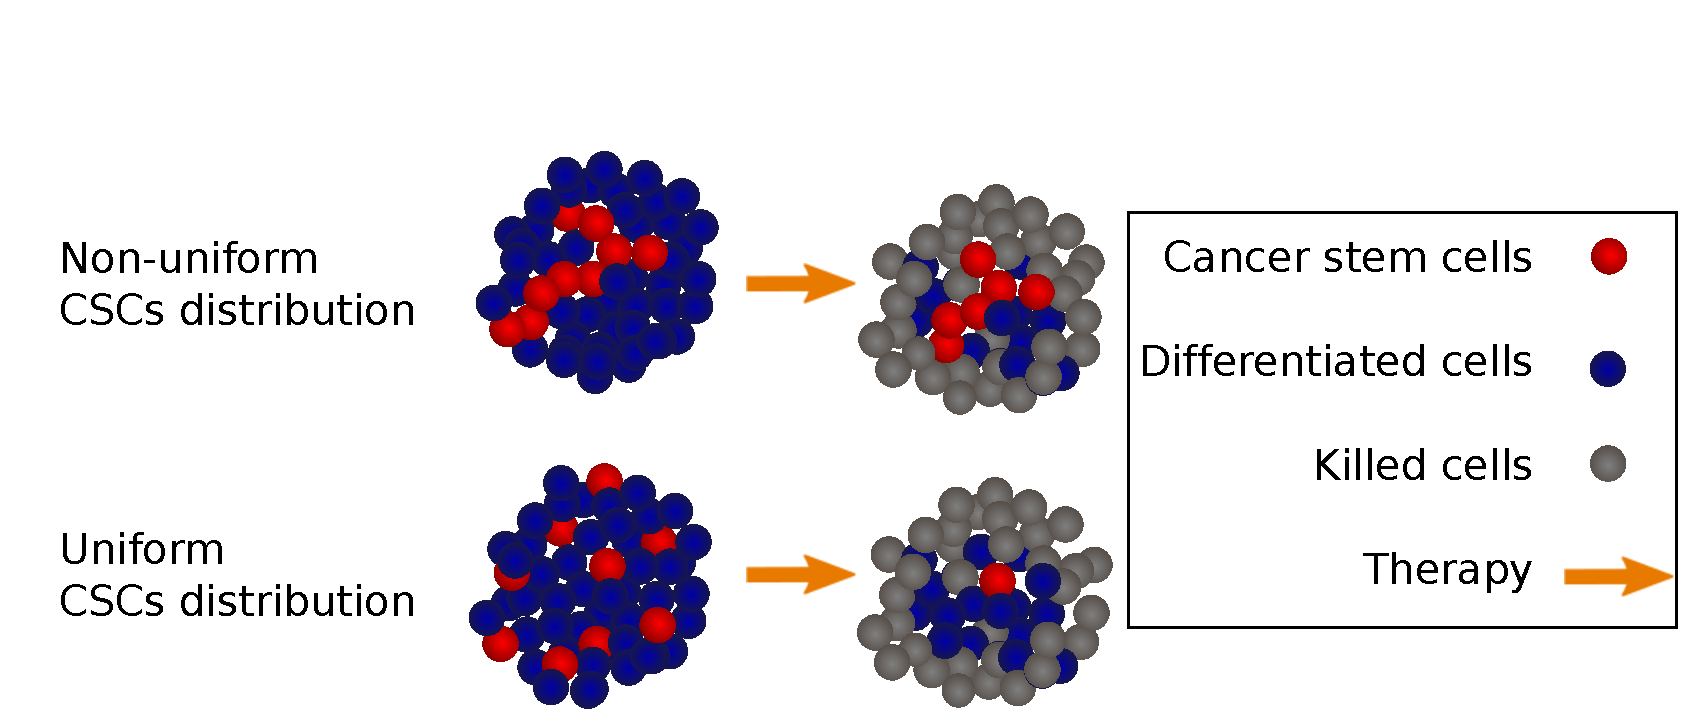
\includegraphics[width=\linewidth]{./images/grabs}
\end{graphicalabstract}

%%Research highlights
\begin{highlights}

\item Computational model predicts cancer stem cell (CSC) distribution in tumorspheres.

\item CSCs are predominantly located in the central regions of the tumorspheres.

\item Their non-uniform spatial distribution contributes to their radioresistance.
 
\item Understanding CSC location is crucial for experiment design and therapy optimization.
 
\item Results are not substantially modified by the emergence of necrosis.
\end{highlights}

\begin{keyword}
%% keywords here, in the form: keyword \sep keyword
Cancer stem cell \sep Radioresistance \sep Tumorsphere \sep Oxygen availability \sep Necrotic core \sep Cell location
%% PACS codes here, in the form: \PACS code \sep code

%% MSC codes here, in the form: \MSC code \sep code
%% or \MSC[2008] code \sep code (2000 is the default)

\end{keyword}

\end{frontmatter}

%% \linenumbers

\section{Introduction}

The development of many solid tumors is determined by the presence of cancer stem cells, cells that may self-renew and differentiate, giving rise to the differentiated cancer cells (DCCs) that make up the bulk of the tumor \cite{baccelli2012evolving,batlle2017cancer,jagust2019metabolism}. Tumor recurrence and metastasis have been attributed to a special ability of the CSCs to resist cytotoxic drugs and radiotherapy \cite{kreso2014self,batlle2017cancer,prieto2017drug,la2018explaining,malta2018machine,feng2020,bhattacharya2020smar1}. The prevailing view is that surviving CSCs are critical drivers of tumor relapse and metastatic spread. Consequently, effective therapeutic strategies must specifically target CSCs or their supportive microenvironments. To achieve this, it is crucial to identify the spatial distribution of CSCs within tumors and to understand the mechanisms underlying their resistance to therapy. Three key features are known to contribute to the exceptional radioresistance of CSCs: low levels of reactive oxygen species (ROS), enhanced DNA damage repair capacity, and quiescence \cite{Bao2006, Skvortsova2015, Arnold2020}. In this work, we identify a fourth contributing factor to CSC radioresistance: their spatial localization within the tumor. Specifically, we show that CSCs accumulate in hypoxic (poorly oxygenated) regions, which renders them less sensitive to radiotherapy. Our results demonstrate that the resistance of CSCs to radiation is strongly influenced by their preferential positioning away from the surface. 

The first step is to determine where the CSCs are located prior to the therapy. We work with tumorspheres, spheroids grown in suspension from a single cancer stem cell  \cite{gu2011effect, chiodi2011drug,yang2013three, weiswald2015spherical, lee2016tumorsphere, benitez2019, benitez2021, barberis2021, Fotinos2023}. In a recent experiment \cite{fotinos2024}, tumorspheres enriched in CSCs were cultivated, and the immunofluorescent detection of the stemness marker SOX2 was carried out using confocal microscopy. An image processing method that reconstructs the number and location of the CSCs in the spheroids was then implemented; this analysis revealed that, consistent with the predictions of a two-dimensional model \cite{barberisRadialPercolationReveals2021}, CSCs accumulate in the interior of the spheroid. However, we note that the findings of Ref. \cite{barberisRadialPercolationReveals2021} are not straightforward to generalize to three dimensions, where the increased number of available growth paths could a priori substantially modify the spatial distribution of CSCs. Therefore, in order to realistically simulate tumorsphere growth, it is necessary to extend the existing model to three dimensions. Computationally, we start from a single CSC seed and, consistent with the observations of Brú and co-workers \cite{bru2003}, and of Enderling, Hlatky and Hahnfeldt \cite{enderling2009}, allow it and its progeny to either duplicate or generate DCCs provided there is sufficient space for the newly produced cells. The resulting spheroids contain a core of stem and non-stem quiescent cancer cells, unable to proliferate, and a rim of proliferative cells.

We also need to describe how the local oxygen availability conditions cell survival. It has been known for many years that hypoxic tumor cells are less sensitive to radiation than well-oxygenated ones \cite{grimes2016role}. In fact, reoxygenation of tumor cells may increase tumor control \cite{kim2005repopulation}. This oxygen enhancement of the radiation effects is attributed to the oxygen-induced fixation of DNA damage \cite{grimes2015mechanistic}. In embryonic stem cells hypoxia is negligible for aggregates with a radius smaller than 100 $\mu m$, but it becomes an important factor for aggregates larger than 300 $\mu m$ \cite{wu2014oxygen}. Of course, these numbers depend on the cell line, the environment, and on the spheroid tortuosity and porosity. A mathematical model to describe the role of oxygen in avascular tumor growth was developed in Refs. \cite{grimes2014method,grimes2015mechanistic} and used by Brüningk and coworkers to investigate spheroid response to radiation therapy \cite{bruningk2019}. Here we will follow Frieboes and co-workers and assume that oxygen consumption grows linearly with the oxygen concentration, i.e., that consumption is far from saturation \cite{frieboes2006}. We will also assume that the probability of cell killing is proportional to the absorption of oxygen. This probability will be taken to be the same for CSCs and DCCs, so that any differences we find in phenotype survival can be solely attributed to the cell location at the time the radiotherapy is applied.

In a standard experimental assay, it is possible to determine the Population Doubling Time (PDT) of the total cell population. Since this measurement cannot discriminate between the growth rates of CSCs and DCCs, we will assume the same intrinsic growth rate for both populations  \cite{benitez2021}. The reproduction of CSCs displays three options: they can self-renew, yielding two CSCs, with a probability $p_s$, they can yield two DCCs with a probability $p_d$, or they can reproduce asymmetrically, yielding one CSC and one DCC, with a probability $p_a = 1 - p_s - p_d$. The self-replication probability $p_s$ is small in homeostasis and in most common culture media. Nevertheless, CSCs can be forced to self-renew by changing their microenvironmental conditions, e.g., by using specific growth factors that inhibit differentiation. In these situations, $p_s$ can be close to unity and tumorspheres become enriched in CSCs \cite{wang2016novel,marks2024role}. Thus, $p_s$ is the key parameter regulating the CSC fraction in simulations, mimicking the effect of growth factors in tumorsphere assays. To simplify the analysis, we will neglect $p_d$, an approximation that will not result in any substantial changes.

Detailed mathematical models of the early phases of CSC-driven tumor growth and the effects of radiation have been developed over the last 15 years, primarily by H. Enderling and collaborators \cite{enderling2009, enderling2009a, gao2013, enderling2015, poleszczuk2015}. Among their findings, is the observation that radiation enriches the CSC population, potentially leading to accelerated tumor repopulation. This phenomenon occurs as quiescent tumor cells may opportunistically proliferate into space freed by radiation-induced cell killing \cite{enderling2009a, gao2013}. They termed this effect a paradox and further explored its implications for tumor invasiveness \cite{shyntar2022}. They also predicted that varying the DCC proliferation capacity (that is, the length
of differentiated progeny after a CSC generates a DCC) leads to different growth kinetics \cite{enderling2011, morton2011, poleszczuk2015}. Their models, intended for in vivo tumors,   predict that CSCs should be predominantly concentrated in the interior of the tumor, as illustrated, for instance, in Fig. 2 of Ref. \cite{gao2013}.  We note that a phenomenon similar to the radioresistance paradox has also been described in the context of chemotherapy \cite{menchon2011}. In the field of proton radiotherapy, Schniewind and co-workers investigated the role of cellular plasticity in tumor growth and response to treatment. They found that ionizing radiation can enrich the population of aldehyde dehydrogenase (ALDH)-positive CSCs, a subpopulation associated with increased tumorigenicity and resistance to therapy \cite{schniewind2022}.

Since our focus is to simulate experimental radiation on tumorspheres, which lack  long-term dynamics, we adopt a deliberately simplified model. This approach allows us to isolate and examine the relationship between the spatial distribution of cancer stem cells and radioresistance, without introducing additional effects that are nonessential at early times and could obscure our primary objective. 

 Our working hypothesis is that an important reason for the observed survival of a higher fraction of CSCs than DCCs is the concentration of CSCs in the most hypoxic region of the tumorsphere. In this paper we verify the validity of this hypothesis using a computational growth model. We begin by presenting simulation results that describe the evolution of the CSC distribution in a growing tumorsphere, and then analyze the effect of a radiotherapy session on the CSC and DCC populations. We then compare our results with those obtained when spheroids containing random distributions of both subpopulations are irradiated. Finally, the impact of the application of radiotherapy after the emergence of a central necrosis is considered in detail.



%%%%%%%%%%%%%%%%%%%%%%%%%%%%%%%%%%%%%%%%%%%%%%
%                     Methods
%%%%%%%%%%%%%%%%%%%%%%%%%%%%%%%%%%%%%%%%%%%%%%
\section{Methods} \label{section: methods}

\subsection{Overview of the Computational Model}

We use a tailored Python 3 object-oriented code, built as a package (see \href{https://github.com/JeroFotinos/tumorsphere_culture}{\lstinline|tumorsphere_culture|}), with cells in two \emph{phenotypes}: CSCs and DCCs. Each cell can be either in a \emph{proliferative} or a \emph{quiescent} state during growth, and change to a \emph{killed} state after radiotherapy. We start the simulation with one active CSC and ask it to duplicate. Later, at each time step, we ask all proliferative cells to divide, provided there is enough room for the new cell. Cells that fail to proliferate on account of the lack of space change to the quiescent state. If there is enough room and the replicating cell is a CSC, it either self-renews with a probability $p_s$ or generates one CSC and one DCC with a probability $1-p_s$. If the parent and daughter cells belong to different phenotypes (one CSC and one DCC), we exchange the positions of the original CSC and the new DCC with a probability $1/2$. Naturally, an active DCC can only create another active DCC, so in this case, the switching would be inconsequential. We remark that the model is lattice-free. Although the model is lattice-free, for computational efficiency we used a custom discretization inspired by the Moore neighborhood, designed to preserve the generality of the approach. Updates are made in random order; once all the proliferative cells are requested to duplicate, independently of the success of their attempts, we say that a one-day-long time step has been performed. This implies, without any loss of generality, that the PDT is one day, corresponding to a reasonable growth rate that also aids intuition. Further details on the structure of the simulation process are reported in \cite{barberisRadialPercolationReveals2021}. We note that, by neglecting the probability of symmetric differentiation, we are considering the most favorable case for CSC expansion. If symmetric differentiation were allowed, fewer CSCs would be found near the tumorsphere's surface, further reinforcing our results.

\subsection{Package Architecture}
We have a class for cells, a class for cultures, and a class for simulations. \lstinline|Simulation| objects coordinate the evolution of \lstinline|Culture|'s. In turn, \lstinline|Culture|'s are collections of \lstinline|Cell|'s. In both cases there is an aggregation relationship. However, while \lstinline|Culture|'s can be instantiated by \lstinline|Simulation|'s or on its own, \lstinline|Cell|'s are components that can only exist as part of their container (\lstinline|Culture|'s). The simplest simulation one can make, requires a \lstinline|Culture| with its \lstinline|cells|, \lstinline|grid|, and \lstinline|output|. Optionally, one can orchestrate many realizations at a time with a \lstinline|Simulation| object, say for a parameter sweep. Therefore, there is a composition relation between \lstinline|Cell|'s and \lstinline|Culture|'s, and only an aggregation relationship between \lstinline|Culture|'s and \lstinline|Simulation|'s. This is illustrated in Fig. \ref{fig: uml_classes}. It is worth mentioning that the \lstinline|Cell| class is actually a data class, due to memory efficiency considerations. That is why there are no methods in this class, and all cell behavior is managed by the \lstinline|Culture| class.

\lstinline|DatOutput|, \lstinline|OutputDemux|, \lstinline|OvitoOutput|, and \lstinline|SQLOutput| implement the interface given by the abstract class \lstinline|TumorsphereOutput| via inheritance. They are in charge of storing the simulation results in different ways, changing the output's format and the amount of detail included in the output. Broadly speaking, \lstinline|DatOutput| is the least detailed result one can get from simulations, providing only the number of cells of each kind as a function of time. At the other end of the specturm, \lstinline|SQLOutput| is the most complete output and registers everything that happens in a simulation into an SQL database, from the parent of each cell, to the time at which a particular cell deactivated. \lstinline|OvitoOutput| is used to produce data in the appropriate format for rendering the culture's evolution. \lstinline|OutputDemux| allows combining many different output types, delegating each task to its list of requested output objects. In that way, a \lstinline|Culture| object can use both \lstinline|DatOutput| and \lstinline|OvitoOutput| at the same time. \lstinline|TumorsphereOutput| objects always exist as components of a \lstinline|Culture| object, so we have again a composition relationship.

The \lstinline|SpatialHashGrid| class manages the grid-based spatial hash. The basic idea is to divide the 3D space into cubes of a given size, and see in which of them a given cell lies. Then, when looking for overlaps between cells, we only have to check the distances with the cells in the same cube of the original cell, or the neighboring cubes. This greatly enhances performance and allows simulating cultures with a high number of cells. \lstinline|SpatialHashGrid| objects always exist as components of a \lstinline|Culture|, their aggregation relationship following from that. There's also a dependency between \lstinline|Simulation| and \lstinline|SpatialHashGrid| due to direct mention of the latter's name in the former.


\begin{figure}
	\centering
	\includegraphics[width=1.0\textwidth]{./images/classes.pdf}
	\caption{\emph{UML diagram for the package's classes.} \lstinline|Simulation| objects are aggregates of \lstinline|Culture| objects, and \lstinline|Culture| objects are composed by \lstinline|Cell| objects. \lstinline|DatOutput|, \lstinline|OutputDemux|, \lstinline|OvitoOutput|, and \lstinline|SQLOutput| implement the \lstinline|TumorsphereOutput| interface. \lstinline|TumorsphereOutput| and \lstinline|SpatialHashGrid| objects always exist as components of a \lstinline|Culture| object, so we have again a composition relationship between them and the \lstinline|Culture| class. The \lstinline|Simulation| class depends on the \lstinline|SpatialHashGrid| class, since the latter is instantiated by the former when creating \lstinline|Culture|'s. }
	\label{fig: uml_classes}
\end{figure}

\subsection{Implementation of Therapy}

We implement a simple model of radiotherapy: a single dose is uniformly applied and the fraction of killed cells (CSCs and DCCs) is assumed to depend only on the local oxygen consumption rate and not on the cell stemness. 
For small tumorspheres, we could assume that the oxygen distribution is uniform, but for larger tumorspheres, we must compute it using the diffusion equation, obtaining a concentration that depends on the distance from the spheroid center. The $O_2$ concentration is rescaled in such a way that it takes the value of unity at the spheroid edge and may thus be compared to a probability density. Then, we model the effect of the therapy by killing cells with a probability $1-c(r)$, where $c(r)$ is the concentration of $O_2$ at a distance $r$ from the cell center.  In each simulation run, we select a number at random between 0 and 1. If this number is larger than the local value of the oxygen concentration, the cell survives; otherwise, it dies immediately. Finally, we group the numbers of total (t), surviving (s), and killed (k) cells of each phenotype (CSC and DCC) in 10$\mu m$-thick -a cell diameter- spherical layers to generate histograms and measure the required fractions. 
Since our primary interest lies in the effect of the spatial distribution of the CSCs on radioresistance, the overall dependence on radiation dose is not central to our analysis and will be neglected. Nevertheless, the Linear-Quadratic (LQ) model can be readily adapted to investigate the influence of radiation dose $D$ on cell survival. Notably, the survival fraction, $SF(D)$, predicted by the LQ model does not incorporate spatial information \cite{chadwick1973molecular,buffa2000analysis,bruningk2019}. Therefore, if the relative effect of dose on overall survival is of interest, it can be approximated by multiplying the spatially resolved total concentration of surviving cells, $S(r)$, obtained from our model by the $SF(D)$ derived from the LQ model.




\subsubsection{Modelling $O_2$ Uptake}

Since we will assume that cell sensitivity to radiation is controlled by oxygen absorption, we need to know the oxygen distribution inside the tumorsphere. This distribution depends on the rate of oxygen uptake. Various forms have been proposed for the dependence of oxygen uptake on oxygen concentration. Some authors use zero-order kinetics (absorption rate independent of local concentration) \cite{chow2001modeling, cai2013hybrid,grimes2016role}, while Frieboes and co-workers use first-order kinetics (oxygen uptake proportional to the local concentration) \cite{frieboes2006}. Other authors use saturation-type kinetics of the Michaelis-Menten \cite{wu2014oxygen} or exponential \cite{scalerandi1999nutrient} forms. Since we are interested in considering regions with low oxygen concentrations, for which concentration-independent uptake is not a good approximation, we choose first-order kinetics. The oxygen distribution in small tumorspheres is approximately constant, but in medium-sized or large spheroids, the concentration decreases substantially as we move away from the surface. We thus need to consider oxygen diffusion and uptake inside the spheroid. Since oxygen diffusion occurs over much shorter timescales than cell replication, the oxygen distribution $c(r)$ can be assumed to satisfy the steady state diffusion equation at all times,
\begin{equation}
	L^{2} {\bigtriangledown}^{2}c = c
\end{equation}

where $L$ is the diffusion length,

\begin{equation}
	L = \sqrt{(D/\mu)} 
\end{equation}
Here $D$ is the oxygen diffusion coefficient and $\mu$ is the oxygen absorption rate, which is assumed to be the same for CSCs and DCCs. As mentioned before, we fix the oxygen concentration at the tumorsphere boundary to unity, i.e., $c(r = R(t)) = 1$, with $R(t)$ being the instantaneous tumorsphere radius. Since the tumorsphere maintains an approximately spherical geometry throughout its evolution, we define $R(t)$ as the average radial distance of all non-quiescent cells from the spheroid center. The second boundary condition is ${dc}/{dt}{\mid}_{r=0}=0$.

The value of the diffusion length may be found by considering the thickness of the viable rim. In this work, we take $L=100 \mu m$. The derived boundary value problem is solved numerically by means of a 4th-order collocation algorithm, as implemented by \href{https://docs.scipy.org/doc/scipy/reference/generated/scipy.integrate.solve_bvp.html#id4}{scipy.integrate.solve\_bvp} (see also \cite{2020SciPy-NMeth}), and using a mesh of 50,000 nodes, which ensures high precision even for large spheroids. 
We then simulate the application of a {\bf single, uniform dose of radiation,} whose effect is to destroy a fraction of the cells that depends on the applied dose and on the local oxygen concentration. Since the dose D is applied uniformly, we may factor out its dependence on D and assume that the total concentration $S(r)$ of surviving cells obeys the equation,

\begin{equation}
	S(r) = 1- c(r). 
\end{equation}

We emphasize that, in our model, radiation is assumed to affect stem and non-stem cancer cells in exactly the same way. To isolate the impact of the spatial distribution of CSCs, we deliberately assume that CSCs and DCCs have the same intrinsic sensitivity to therapy. It is also convenient to describe the cell distributions inside the tumorspheres using histograms, which average the results over 32 realizations, and whose bins, with width  $a = 10 \mu m$, give the probability of finding a cell between $r$ and $r+a$, with $r$ being the distance from the spheroid center. In this way, the functions interpolating each histogram (obtained through a Kernel Density Estimation-KDE) represent the probability density of finding a cell of the given class at a distance $r$ from the spheroid center. 


\subsubsection{Random CSC Distributions}
The non-uniform spatial distributions of CSCs we obtain are a direct consequence of the choices that CSCs make when they proliferate, and of space constraints. To address the protective nature of the CSC location, we compare the effect of radiotherapy on tumorspheres generated with our model with its effect on spheroids containing random distributions of CSCs. The latter were built by first taking the tumorspheres described in previous sections and removing the labels that distinguish between cell phenotypes. Then, for each of these ``plain'' tumorspheres, we randomly assign the CSC phenotype to the cells in such a way that they end up with the same number of CSCs as the original spheroids. Finally, we apply the therapy and collect the distributions of surviving and killed cells in each phenotype as described in previous sections. We repeat this redistribution and therapy process 50 times on each plain tumorsphere to increase the statistical confidence of this study. Comparing the outcomes of radiotherapy applied to model-generated versus random CSC distributions allows us to isolate the impact of spatial geometry on effective CSC radioresistance.


\subsubsection{Tumorspheres with Necrotic Core}
As shown by Freyer \cite{freyer1986}, cells in the inner regions of spheroids die due to low oxygen pressure, leading to the formation of a necrotic core surrounded by a viable rim of living cells. A central necrosis typically appears once spheroids reach diameters of approximately $500-800$ $\mu$m. Although the thickness of the viable rim was once assumed to remain constant with spheroid growth, it is now recognized that in many cases the rim thins as the diameter increases \cite{Groebe1996}. Some models describing the development of this necrotic core assume that oxygen is completely consumed in the outer rim, imposing a zero-flux condition at the necrotic core-viable rim boundary \cite{Burton1966, grimes2014method}. Since, from a mechanistic standpoint, necrosis is primarily driven by oxygen depletion, we assume instead that cells die when the local oxygen concentration drops below a threshold value, while maintaining the zero-flux boundary condition at the tumorsphere center. Because CSCs exhibit greater plasticity to adapt to hypoxic conditions \cite{ mimeault2013, iriondo2015, carnero2016, papale2020}, we assign different hypoxic thresholds, $c_S$​ and $c_D$, to the CSC and DCC phenotypes, respectively, with $c_S < c_D$​. Tumorspheres are then grown as in previous cases, but all cells with oxygen concentrations below their respective thresholds are defined as \emph{dead}. We also define the necrotic core radius, $R_n$​, as the maximum distance from the spheroid center at which viable DCCs are still present.


\section{Results}

In this section we present the cell phenotype distributions in tumorspheres, before and after the application of a single, uniform radiation dose. Successive applications are outside the scope of this study, as our goal is not therapy design but the effect of spatial cell distributions. We therefore present histograms of cell spatial distributions, stratified by phenotype.  As explained in the Methods section, the functions interpolating each histogram (see section \ref{section: methods}, Methods) represent the probability density of finding a cell of any phenotype at a distance $r$ from the spheroid center. For comparison, in the following subsection, we also present the results of the therapy application to spheroids where the cells of both phenotypes have been randomly distributed in their interior. In the last subsection, we study the effect of radiation on tumorspheres with a necrotic core.


\subsection{Phenotype distribution in a tumorsphere}

Typical outcomes of the growth process in the absence of a necrotic core are shown in Fig.\ref{f:methods} for $p_s = 0.4$, a value found compatible with the U87-MG cell line \cite{gao2013} and $p_s = 0.7$ (a CSC-enriched system) after simulating for 30 days (30 time steps), a relatively long period for a tumorsphere experiment. To better track the subpopulations present in the tumorsphere, proliferative CSCs are colored in  red and proliferative DCCs in blue; the colors of the quiescent cells in each phenotype are lightened. The result for $p_s = 0.4$ is depicted in panel \ref{f:methods}a, where a cut of the tumorsphere shows that the CSCs are all quiescent, trapped near the center of the colony, and surrounded by DCCs. For $p_s = 0.7$, panel \ref{f:methods}b shows that there are CSCs in a proliferative state at the colony surface; they appear at the surface as red spots surrounded by proliferative DCCs (panel \ref{f:methods}c). This is significant, given that most mathematical models in the literature assume a uniform CSC distribution. Furthermore, we carried out some preliminary experiments \cite{fotinos2024}, confirming that the CSC distribution looks as predicted by the model, an agreement that highlights the power of simulations to guide experiments.

% ==== FIG 1 ====
\begin{figure}
	\centering
	\includegraphics[width=\textwidth]{./images/F1.eps}
	\caption{(a) Sagittal cut of a tumorsphere for moderate self-renewal probability ($p_s=0.4$). CSCs are quiescent and confined to the core.  (b) Sagittal cut for high self-renewal probability ($p_s=0.7$). CSCs have a chance to reach the border and keep proliferating. (c) External view of the tumorsphere for large self-renewal, showing  proliferating CSCs (in red) at the surface. (d) Time evolution of CSC populations. For $p_s=0.4$ (blue) the growth of CSCs is arrested at an early stage. For $p_s=0.7$ the population of CSCs keeps increasing but its growth rate decreases over time.  (e) Oxygen profile as a function of the distance $r$ from the center for 10-day (blue) and 30-day (orange) tumorspheres.   (f) Total cell distribution inside a 30-day tumorsphere ($\rho$ is the number of cells in each shell).  \label{f:methods}} 	
\end{figure}

% ====== TABLA ======
\begin{table}[htbp]
	\centering
	\caption{Cell population statistics for 30-day tumorspheres ($p_s=0.7$ everywhere). The total population (t) of cells is broken down by phenotype (CSCs and DCCs) and by killed (k) and surviving (s) cells. }
	\label{table}
	\begin{adjustbox}{width=\textwidth} % This will make the table fit within the page width
		\begin{tabular}{||l || r | r || r |r||}
			\toprule
			{} & \multicolumn{2}{c|}{without necrosis}  & \multicolumn{2}{c|}{with necrosis}  \\ \cline{2-5}
			{} & model & random & model & random \\
			\midrule
			tCells & 27088  &27088  & 27088  & 27088 \\
			tCSCs & 1999  & 1999 & 1999 & 1999 \\
			tDCCs & 25089   & 25089 & 25089  & 25089 \\ \midrule
			sCells & 13397  & 13397 & 8377&  8377\\
			sCSCs & 1169 & 986 & 794  & 618 \\
			sDCCs &  12227  &  12410 & 7583 & 7758 \\  \midrule
			kCells & 13691& 13691 & 18710 & 18710\\
			kCSCs & 829  & 1012 & 1204 & 1380 \\
			kDCCs & 12862 &  12678 &  17506 & 17330\\ \midrule
			Pre-therapy CSC Fraction & 0.073 & 0.073& 0.073 & 0.073\\
			Post-therapy CSC Fraction & 0.087 & 0.073 & 0.094 & 0.074\\ 
			CSC increase & 1.191 & 1.000 & 1.287 & 1.014 \\ 
			\midrule
			kCSCs / tCSC & 0.415 &  0.507 & 0.602&  0.690\\
			kCSCs / kCells & 0.061&  0.073& 0.064& 0.074 \\
			kCells / tCells & 0.505 & 0.504 & 0.691 & 0.691  \\
			kDCCs / tDCC& 0.512 & 0.505& 0.698 & 0.691 \\
			\bottomrule
		\end{tabular}
	\end{adjustbox}
\end{table}


The evolution of the total number of CSCs is shown in Fig. \ref{f:methods}d for an average over 32 realizations of the 30-day-old tumorspheres. As expected, the fastest growth in the CSC number occurs for the highest $p_s$. Growth is arrested earlier for $p_s = 0.4$ (blue line), because CSCs become rapidly surrounded by DCCs. In the case of the larger self-renewal probability ($p_s = 0.7$, orange line), CSCs continue to proliferate for longer times, but their growth rate decreases monotonically. Ongoing physical analysis using percolation theory surprisingly indicates that, if the tumorsphere were allowed to grow indefinitely, at very long times CSCs would appear at the surface only if there were no differentiation ($p_s=1.0$). Thus, for $p_s<1$, it is unlikely, although theoretically possible, to find CSCs on the surface of large spheroids. Figure \ref{f:methods}e shows the oxygen profiles for 10-day-old (blue) and 30-day-old (orange) tumorspheres. The low oxygen concentration near the center of the bigger tumorspheres makes cells there especially radioresistant.

Because of the geometrical constraints, the tumorspheres have their cells roughly distributed in layers. In Fig. \ref{f:methods}f we depict the radial distribution of the cells of both phenotypes in $10 \mu m$-thick layers for a 30-day-old tumorsphere. At the center of the tumorsphere, there is only the initial cell. As we move away from the center, the area of the layers increases as $r^2$. As a consequence, more cells have room to proliferate and the proliferative phenotype predominates in the outer layers. In this region, the cells cannot fill the layers during the same timestep, and the number of cells per layer decreases.  The CSC distribution is flattened and shifted toward the center because DCC creation and space restrictions hinder their growth, while the DCC distribution has many more cells near the surface.
      



%%%%%%%%%%%%%%%%%%%%%%%%%%%%%%%%%%%%5
%% small
%%%%%%%%%%%%%%%%%%%%%%%%%%%%%%%%%%%

\subsection{Radiotherapy on Small Tumorspheres}

In Fig. \ref{f:dosis_const}, we show histograms for 10-day-old tumorspheres, where $\rho_S$ and $\rho_D$ are, respectively, the average numbers of stem and differentiated cancer cells in each shell. The average number of CSCs before the therapy is about half that of DCCs (143 versus 319, respectively) and is slightly dominant near the tumorsphere center, while the DCCs are more abundant near the rim, as shown in  panel (a). In panel (b), we show the surviving and killed cell distributions. Since the cells are well oxygenated everywhere in the spheroid, most cells of both phenotypes are killed and the protection offered by the remoteness from the surface is minimal: as a consequence of the therapy, the percentage of live CSCs had only a small increase: from 30.8\% to 33.2\%. The fraction of surviving CSCs (0.147) is barely higher than that of DCCs (0.135). The distributions of killed cells of both phenotypes are slightly biased towards the outer region. 

% ==== FIG 2 ====
\begin{figure}
	\centering
	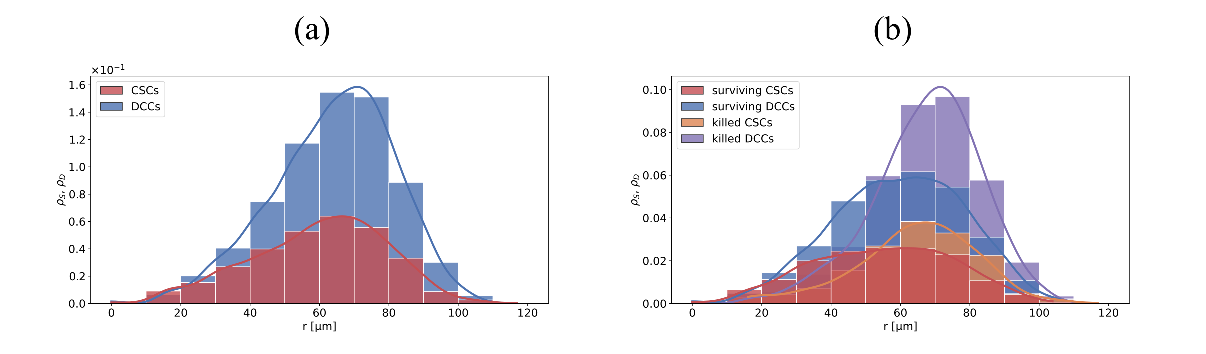
\includegraphics[width=\textwidth]{./images/F2.eps}
	\caption{\emph{Normalized cell distributions for 10-day-old tumorspheres.} (a) Before therapy, CSCs (red) and DCCs (blue) exhibit similar spatial distributions, although the DCCs are slightly displaced outward from the center. (b) Following therapy, few cells of either phenotype remain, a consequence of the high oxygenation of the entire tumorsphere.  The spatial distribution of killed cells closely resembles that observed prior to treatment.}
	\label{f:dosis_const}
\end{figure}




%%%%%%%%%%%%%%%%%%%%%%%%%%%%%%%%%%%%%%%%%%%%%%%%%%%%%%%%
% 30 day
%%%%%%%%%%%%%%%%%%%%%%%%%%%%%%%%%%%%%%%%%%%%%%%%%%%%%%%%
\subsection{30-day Tumorspheres}\label{ss:30-day}

We have shown that, for early-stage tumorspheres, location is not important for CSC survival. The situation undergoes substantial changes when we consider bigger tumorspheres.
Figure \ref{f:30} shows histograms for 30-day-old tumorspheres immediately after therapy. The average number of CSCs before treatment was 1,999, from which 1,169 (58.5 \%) survived, whereas 12,227 (48.7 \%) from the original 25,089 DCCs survived. The CSC fraction of the total cell number, which was 0.073 before the therapy, grew to 0.087 afterward (see Table \ref{table}). Figure \ref{f:30}a displays the distribution of cells of each phenotype as a function of the distance from the tumorsphere center. A large fraction of the DCCs were killed near the surface, and the peak of the surviving DCC distribution was truncated due to the large number of DCCs killed near the rim. Because the number of DCCs is much larger than that of CSCs, the CSC distributions are magnified in Fig. \ref{f:30}b. The black line represents the KDE for the total CSC population, which has a relatively flat profile and drops off at $r=290 \mu m$, close to the maximum of the DCCs distribution. After therapy, the total CSC distribution separates into two well-defined peaks. The peak of the surviving CSC distribution (red) shifts toward the center while maintaining a relatively flat profile, whereas the peak of the killed CSC distribution (orange) shifts toward the surface. This distribution exhibits an approximately linear increase with the radius in the region to the left of the maximum. A comparison of panels (a) and (b) shows that, while the maxima of the surviving cell distributions are well separated, those of the killed cell distributions coincide. A different perspective emerges if we look at the radial dependence of the cell densities depicted in Fig. \ref{f:30}c. For both killed and surviving CSCs, the density  decreases with increasing radius, reflecting their  abundance in the tumorsphere core. In contrast, the density of killed DCCs (violet) increases towards the surface, due to the pre-therapy DCC predominance there. The protective nature of the outer rim is further evidenced by the radial density of surviving DCCs (blue), which has a flattened maximum  far from the surface.  For clarity, Fig. \ref{f:30}d shows the fractions of each type of cell as a function of the distance from the tumorsphere center.  The fraction of surviving cells for both  phenotypes is similar near the center, but decays with radius for the CSCs. In the outer rim, the fraction of killed cells is close to one, with most of them being DCCs. This last panel confirms the self-renewal/differentiation mechanism as key to the resistance of CSCs to radiotherapy.

% ==== FIG 3 ====
\begin{figure}
	\centering
	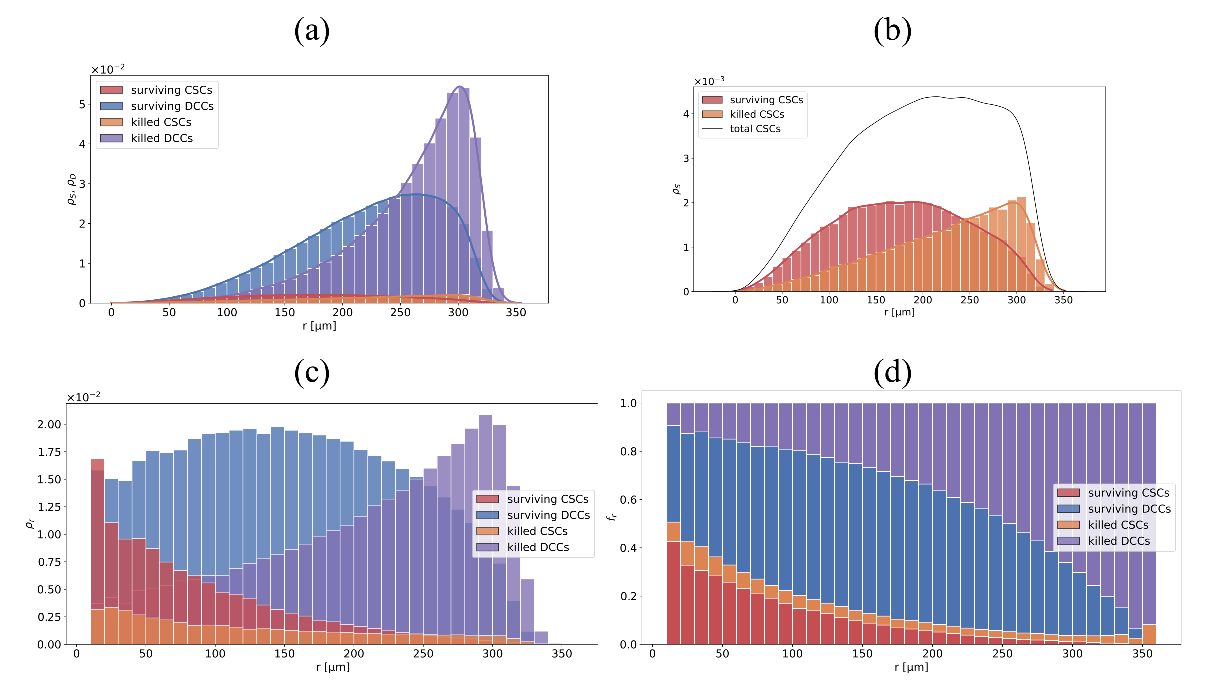
\includegraphics[width=\textwidth]{./images/F3.eps}
	\caption{\emph{Cell distributions for 30-day-old tumorspheres after therapy.}  (a) Killed and surviving CSC and DCC histograms. For both phenotypes, cells were preferentially killed closer to the surface. (b) Expanded view of the distributions of surviving and killed CSCs. (c) Cell density shows CSCs are mainly located far from the surface. (d) Cell fractions reveal that cells are protected in the core of the tumorsphere.}
	\label{f:30}
\end{figure}


%%%%%%%%%%%%%%%%%%%%%%%%%%%%%%%%%%%%%%%%%55
% Random
%%%%%%%%%%%%%%%%%%%%%%%%%%%%%%%%%%%%%%%5
\subsection{Comparison with Random CSC Distributions}

To reinforce our conclusions on the impact of the non-uniformity of the CSC distribution on their survival, we implement the same radiotherapy dose to spheroids obtained from the tumorspheres studied in section \ref{ss:30-day} by redistributing both cell phenotypes at random, as explained in the Methods section. The results are depicted in Fig. \ref{fig:random}, whose panel (a) shows the distributions of surviving and killed CSCs immediately after a therapy application at $t = 30$ days. The histograms for the CSCs and DCCs exhibit the same spatial profiles, albeit at different scales, as seen by comparing with panel (b), which displays the CSC distributions alone. In this panel, we compare the distributions from our model to those resulting from a random distribution of CSCs immediately before the therapy. When the pre-therapy distribution is generated by our model, surviving CSCs are positioned closer to the tumorsphere center than their randomly generated counterparts. They are also noticeably more numerous than those that originated from the random distribution. A complete set of statistical values is reported in Table \ref{table}. These results clearly show that the killed CSC fraction was lower in our model than in the random distribution (41.5\% vs. 50.7\%), while the number of surviving CSCs was 19\% higher. The reason for this difference is that more cells get killed near the rim, where the $O_2$ concentration is high, and where our model predicts fewer CSCs to be located.  


% ==== FIG 4 ====
\begin{figure}
	\centering
	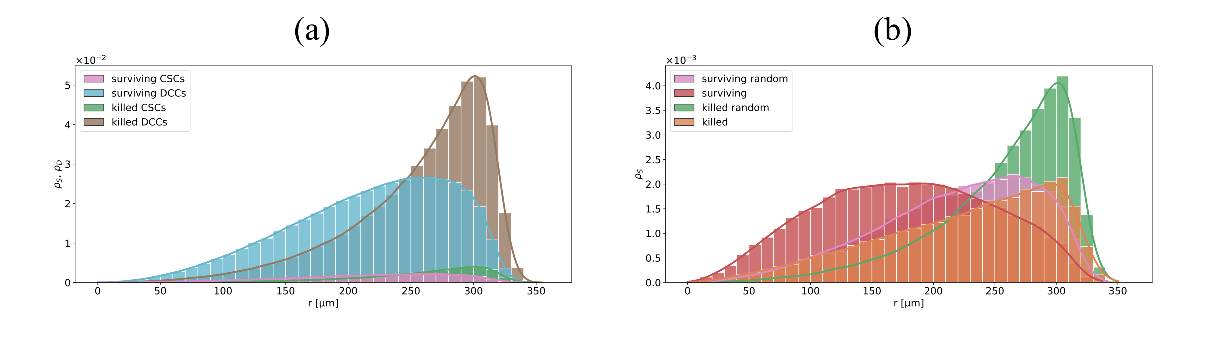
\includegraphics[width=\textwidth]{./images/F4.eps}
	\caption{\emph{Effect of radiotherapy on a 30-day-old tumorsphere with a random CSC distribution.} Histograms show cell numbers as a function of distance from the tumorsphere center. (a) CSC and DCC spatial distributions display the same overall shape, although their total numbers differ greatly. (b) Comparison between the CSC distributions in our model and those resulting from a random cell allocation. The number of surviving CSCs is higher in our model.}
	\label{fig:random}
\end{figure}


%%%%%%%%%%%%%%%%%%%%%%%%%%%%%%%%%%%%%%%%%%%%%%
%                Necrotic Core in t=30
%%%%%%%%%%%%%%%%%%%%%%%%%%%%%%%%%%%%%%%%%%%%%%

\subsection{30-day-old tumorspheres with a necrotic core}


Large tumorspheres typically develop a necrotic core, making it important to assess how such a core influences the results in the previous sections. We do this for 30-day-old simulated tumorspheres, which reach a typical radius of $R=350 \mu m$. The size of the necrotic core depends on various parameters. Here we use the data from Ref. \cite{mukomoto2020}, which reported, for an MCF-7 spheroid with $R=350 \mu m$, a core radius of $R_n=150 \mu m$. We must estimate the values of the cell death thresholds, $c_D$ and $c_S$, which satisfy $c_D > c_S $. From Eq. (1), with our boundary conditions, we obtain $c(r=150 \mu m) = 0.3)$. Thus, we set $c_D = 0.3$, and, since CSC oxygen consumption varies widely \cite{lee2016tumorsphere}, depending on factors such as the cell line, and there is no reliable data on the CSCc fraction, we choose, without loss of generality, $c_S=0.23$. To our current knowledge, there are no reports on the anoxic CSC fraction, if any.  Thus, the chosen values assume there is a non-negligible CSCs fraction that die by anoxia. 

By definition, $R_n$ is the maximum radius within which there are no live DCCs; because $c_D > c_S$, a small number of CSCs may still survive inside the core, but their oxygen consumption will be negligible, so we may calculate the oxygen distribution disregarding this small population, i.e., taking $c(r)=0$ for $r<R_n$.  Under these conditions, we simulated tumorsphere growth and applied a single radiotherapy dose on day 30, as in previous cases. The cell distribution immediately before therapy is shown in Fig. \ref{fig:necrotic}a, where the necrotic core has reached a radius of $R_n = 150 \mu m$ -visible as the transition between dead (cyan) and live (blue) DCCs. CSCs survive hypoxia within the core, down to about $70 \mu m$ (see inset for a magnified view of this region). Varying $c_S$ merely shifts the boundary between dead and live CSCs. The chosen value for $c_S$ is very conservative as it results in the killing of many CSCs near the center leading to their complete annihilation in large tumorspheres (sup Fig. S3). As a consequence, our simulated tumorspheres represent the worst possible case from the point of view of our hypothesis. Figure \ref{fig:necrotic}b shows that therapy yields the same distribution profiles as in the case without a necrotic core, cf. Fig. \ref{f:30}, except for the truncations due to necrosis. The number of therapy-killed DCCs and CSCs remains in the same proportions as in Fig. \ref{f:30}c. As in Fig. \ref{f:30}b, live CSCs outnumber dead CSCs near the center (the opposite occurs for DCCs). The convex profile of killed DCCs and the concave profile of live DCCs are likewise preserved.

As shown in Table \ref{table}, the average number of CSCs before treatment was 1,999, of which 497 were already in the necrotic core at the time of the irradiation. Subsequently, 707 CSCs were killed by radiation, leaving 794 survivors that represent 39.7\% of the original CSC population. Among the 25089 DCCs present at the time of treatment, 6780 were already necrotized by hypoxia; and 10725 were subsequently killed by radiation. The remaining 7583 DCCs represent 30.2\% of the original DCC population, a significantly lower survival fraction than that of CSCs. The CSC fraction of the total cell population, which would have been 0.073 without hypoxia, rose to 0.076 once the effects of hypoxia were taken into account, and finally increased to 0.094 following therapy, a higher fraction than 0.087, the value predicted in the absence of necrosis (see Table \ref{table}).


To better understand the interplay between radiotherapy and the necrotic core, we divided the number of cells in each radial bin by the area of the corresponding spherical shell to obtain the radial dependence of the cell density. Figure \ref{fig:necrotic}c shows that a higher density of CSCs survives near the tumorsphere center, whereas most DCCs are eliminated by therapy in its periphery. The concentration fraction of each phenotype is presented in Fig. \ref{fig:necrotic}d, with each bar representing the relative abundance of each cell phenotype in a given shell. The inner necrotic core is fully devoid of live cells, while the outer necrotic core contains about 20\% of the CSCs that survived both hypoxia and radiation. In the viable rim ($r > R_n$), DCCs, both dead and alive, are the dominant phenotype, and the CSCs fraction is minimal.
   
Finally, we compare our results with those obtained under the assumption that CSCs and DCCs are randomly distributed over the tumorsphere. In this case, only 618 CSCs survive (see Table \ref{table}), a substantially lower number than the 794 survivors predicted if the CSC spatial distribution is that of our model. Moreover, in the random distribution case, the ratio of the surviving CSCs to the total cell population (0.074) remains unchanged by either hypoxia or radiation.



% ==== FIG 5 ====
\begin{figure}
	\centering
	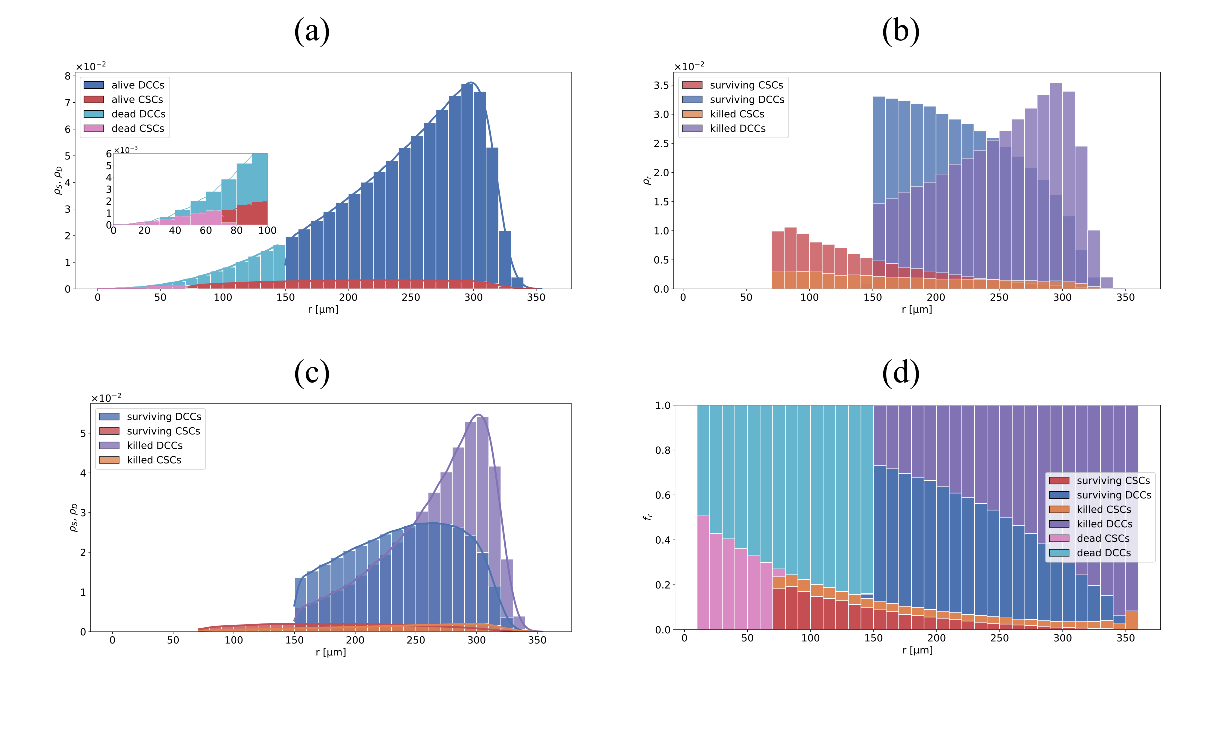
\includegraphics[width=\textwidth]{./images/F5.eps}
	\caption{\emph{Combined effects of hypoxia and radiation on 30-day tumorspheres.} (a) Cell distribution before the therapy. The spheroid has developed a necrotic core of radius $ R_N = 150 \ mu$m. The inset highlights the hypoxic CSC range. (b) Cell distribution after a single dose of radiotherapy; the fraction of killed DCCs in the necrotic core is greater than that of killed CSCs. (c) Histograms from (b) rescaled to show the radial dependence of the cell concentration. (d) Concentration fractions of all cell types. Here $c_S=0.23$ and $c_D=0.30$.}
	\label{fig:necrotic}
\end{figure}


%%%%%%%%%%%%%%%%%%%%%%%%%%%%%%%%%%%%%%%%%%%%%%
%                     Discussion
%%%%%%%%%%%%%%%%%%%%%%%%%%%%%%%%%%%%%%%%%%%%%%
\section{Discussion}

It is well-known that cancer stem cells have a higher probability of surviving radiotherapy than non-stem cancer cells. This outcome is usually attributed to a higher intrinsic radioresistance. In this paper, we showed that the higher CSC survivability is at least partially explained by their location in regions far from the tumorsphere surface, which are also deficient in the oxygen needed to mediate cellular death. To prove our point, we first determined the location of the CSCs within a tumorsphere; this we did by extending a growth model first developed by  \cite{barberisRadialPercolationReveals2021}, whose predictions were corroborated by the experiments of \cite{fotinos2024}. As shown in Fig. \ref{f:methods}, CSCs create paths in the tumorsphere bulk that are eventually frustrated by space limitations that force them into quiescence. As a consequence, most CSCs reside well in the tumorsphere interior. This agrees with the observation by Li and co-workers of CSCs in regions near necroses, which led them to suggest the existence of a hypoxic niche for the CSCs \cite{li2009}.

To focus on the relationship between CSC positioning and survival, we did not consider complicating, but non-essential factors, such as cell shedding \cite{menchon2009modeling}, senescence \cite{gao2013}, or the secretion of toxic molecules that may contribute to limiting spheroid growth. Since our objective is not to model cancer growth, but to analyze the relation between CSC location and survival, we chose the simplest possible description. Radiotherapy was modeled as a single, uniform dose, with the probability of cell killing proportional to the local oxygen concentration $c(r)$, i.e., we assumed that the survival probability is $S(r) = 1-c(r)$, with $c(R) = 1$. This is a very conservative assumption: Killing would be more concentrated near the rim, i.e., away from the CSCs, if, for instance, we assumed (more realistically) that $S(r)=1-ac(r)$, with $a > 1$. This choice would lead to more cells killed near the rim, and thus to an even higher fraction of CSCs among the surviving population. Even with our assumption of only a modest decrease in cell elimination with decreasing oxygen concentration, we showed that the fraction of surviving CSCs is markedly higher than that of DCCs.

Our results were further confirmed by simulating the application of the same radiotherapeutic dose to spheroids obtained by randomly redistributing the CSCs and DCCs inside the tumorspheres, both with and without necrosis. These simulations showed that:
\begin{itemize}
	\item[a)] the surviving CSC fraction is considerably higher in the tumorspheres generated by the model;
	\item[b)] the difference between these survival fractions increases with time, i.e., with tumorsphere size;
	\item[c)] the surviving DCC fraction is slightly higher for the random tumorspheres, as these contain more DCCs near the center, and;
	\item[d)] in the random tumorspheres, the surviving CSC and DCC fractions are essentially equal.
\end{itemize}
Together, these results strongly support our hypothesis that CSC spatial positioning is an important determinant of radioresistance.   

There is a further reason that buttresses our conclusion about the relation between CSC location and survivability. As the spheroid grows, central cells become quiescent and, consequently, consume less oxygen, enhancing radiation resistance. Since CSCs are predominantly positioned far from the surface, quiescence amplifies their chances of surviving the therapy. Because of its structure, our model can also identify which cells become quiescent as the tumorsphere grows. Currently, we are carrying out simulations to quantitatively assess the contribution of quiescence to CSC survival. Since large tumorspheres usually develop a necrotic core, we also modeled the CSC-driven tumorsphere growth under hypoxic conditions, where cells far from the surface die from oxygen deprivation. Due to their greater adaptability to low oxygen levels, some CSCs were allowed to survive within the core. Simulation results indicate that the radiotherapy effects are similar to those observed in non-necrotic tumorspheres. Necrosis is associated with the development of invasion and metastasis \cite{yamamoto2023metastasis}. The survival of CSCs in necrotic regions suggests that the boundary of a necrosis may serve as a niche favorable to plasticity and dedifferentiation. The de-differentiated phenotype has been reported to be particularly common in metastatic tumors \cite{malta2018machine}. These findings reinforce the idea that microenvironmental conditions can shape CSC behavior and, ultimately, tumor aggressiveness.

To test our hypothesis on the role of CSC positioning in radioresistance, we modeled tumorsphere growth as a simplified system initiated from a single cancer stem cell. Although idealized, this approach indicates how spatial organization can affect treatment outcomes, offering insights that may generalize to more complex neoplastic systems. In particular, the observed link between CSC location and survivability could be exploited to optimize radiotherapy, whether applied alone or in combination with other procedures. Of course, translating these findings to real tumors will require models that incorporate additional biological processes such as cell migration \cite{friedl2010}, plasticity \cite{schniewind2022, meacham2013}, and senescence \cite{gao2013, childs2014}. Nevertheless, our results underscore the importance of spatial heterogeneity \cite{junttila2013, tonello2025} in shaping therapy response.



\section{Acknowledgments}

This work was supported by SECyT-UNC (Consolidar project 33620230100392CB) and CONICET (PIP 11220200103005CO). We are grateful to Luciano Vellón for illuminating discussions.
This work used computational resources from UNC Supercómputo (CCAD) – Universidad Nacional de Córdoba (https://supercomputo.unc.edu.ar), which are part of SNCAD, República Argentina.

% --- Bibliography (BibTeX) ---
% Numeric:
\bibliographystyle{elsarticle-num}

% If you want author–year instead:
% \bibliographystyle{elsarticle-harv}

\bibliography{biblio}


% =========================
% Supplementary Materials
% =========================
\clearpage
\part*{Supplementary Materials}
\addcontentsline{toc}{part}{Supplementary Information}

% Reset and prefix counters to "S"
\setcounter{figure}{0}
\renewcommand{\thefigure}{S\arabic{figure}}
\setcounter{table}{0}
\renewcommand{\thetable}{S\arabic{table}}
\setcounter{equation}{0}
\renewcommand{\theequation}{S\arabic{equation}}
\setcounter{section}{0}

\section*{The 60-day-old system}
\addcontentsline{toc}{section}{Supplementary Notes}
To explore the implications of our findings for larger systems we extended the simulations to 60 days, a time when the spheroids had doubled their diameter with respect to their 30-day counterparts. The total cell count, on the other hand, had increased roughly tenfold. On average, these larger spheroids contained 3,668 CSCs, of which 3,364 (91.7\%) survived therapy, and 273,360 DCCs, of which 198,630 (72.7\%) survived (see Table \ref{tab:S1}).

The probability of a CSC being created at the rim decreases with the radius $R(t)$ of the spheroid, since the likelihood of CSCs becoming surrounded by DCCs -and consequently entering quiescence- increases over time. In Fig. \ref*{fig:S1}a, the DCC distributions fall off abruptly near the rim because the outer cell layers are incomplete. This effect can also be observed, albeit less dramatically, in Fig. \ref{f:30}a. The DCC population is substantially larger than the CSC population, which is barely discernible at the bottom of the panel. Figure \ref{fig:S1}b presents a rescaled view of the CSC distributions, showing that very few CSCs are located far from the center and, in particular, at the rim, where they are most likely to be killed. Furthermore, unlike at earlier times, the CSC distribution has developed a rounded peak instead of a flattened profile. Plotting the radial dependence of the cell density (Fig. \ref{fig:S1}c) or the alternate representation (Fig. \ref{fig:S1}d) - further emphasizes that the CSCs are strongly concentrated near the spheroid center, substantially enhancing their survival chances following radiation treatment. 

It is worth remarking that, after a period that depends on the self-renewal probability $p_s$, the position of the CSC peak remains essentially unchanged, while the DCC peak moves outwards, closely tracking the rim. The increasing separation between peaks enhances the relative survival probability of the CSCs, as evidenced by the comparison between Figs. \ref{f:30}b and \ref{fig:S1}b. The density of killed CSC is so low that it is not detectable at the scale of Fig. \ref{fig:S1}d (cf. Fig. \ref{f:30}d), a consequence of the protection conferred to the inner cells by the reduced $O_2$ levels. Since the fraction of surviving CSCs increases with spheroid size, these results underscore the potential advantages of applying radiotherapy at early stages. 

The histograms in Fig. \ref{fig:S2} clearly illustrate the advantages conferred to CSCs by their spatial positioning. Figure \ref{fig:S2}a indicates that the CSC and DCC distributions are similar, differing only in scale. Figure \ref{fig:S2}b shows that far fewer CSCs are killed by radiation when their distribution follows our model (see also Table \ref{tab:S1}).

%\subsection*{Supplementary Note S1. <Title>}
%<Your text> See main text Fig.~2 for comparison.

\section*{Supplementary Tables}
\addcontentsline{toc}{section}{Supplementary Tables}

% ====== TABLE t = 30 vs. t = 60 ======
\begin{table}[htbp]
	\centering
	\caption{Cell population statistics for the cases studied ($p_s=0.7$). The total population (t) of cells is broken down by phenotype (CSCs and DCCs) and by killed (k) and surviving (s) cells. }
	\label{tab:S1}
	\begin{adjustbox}{width=\textwidth} % This will make the table fit within the page width
		\begin{tabular}{l | r | r | r |r}
			\toprule
			{} & \multicolumn{2}{c|}{ 30-day}  & \multicolumn{2}{c|}{60-day}  \\ \cline{2-5}
			{} & heterogeneous & homogeneous & heterogeneous & homogeneous \\
			\midrule
			tCells & 27088  &27088  & 277030  & 277030 \\
			tCSCs & 1999  & 1999 & 3668 & 3668 \\
			tDCCs & 25089   & 25089 & 273360  & 273360 \\ \midrule
			sCells & 13397  & 13397 & 201990& 201990 \\
			sCSCs & 1169 & 986& 3364  & 2678 \\
			sDCCs & 12227  &  12410& 198630 & 199310\\ \midrule
			kCells & 13691& 13691 & 75035& 75035\\
			kCSCs & 829  & 1012 & 303  & 990 \\
			kDCCs & 12862 &  12678 &  74732 & 74045\\ \midrule
			Pre-therapy CSC Fraction & 0.073 & 0.073& 0.013& 0.013\\
			Post-therapy CSC Fraction & 0.087 & 0.073 & 0.016 &0.013 \\ 
			CSC increase & 1.191 & 1.000 & 1.231 & 1.000 \\ 
			\midrule
			kCSCs / tCSC & 0.415 &  0.507 & 0.083& 0.270 \\
			kCSCs / tkCells & 0.061&  0.073& 0.004& 0.0131 \\
			kCells / tCells & 0.505 & 0.504 &0.271  & 0.271  \\
			kDCCs / tDCC& 0.512 & 0.505& 0.273 & 0.270 \\
			\bottomrule
		\end{tabular}
	\end{adjustbox}
\end{table}


\section*{Supplementary Figures}
\addcontentsline{toc}{section}{Supplementary Figures}

\begin{figure}[ht]
	\centering
	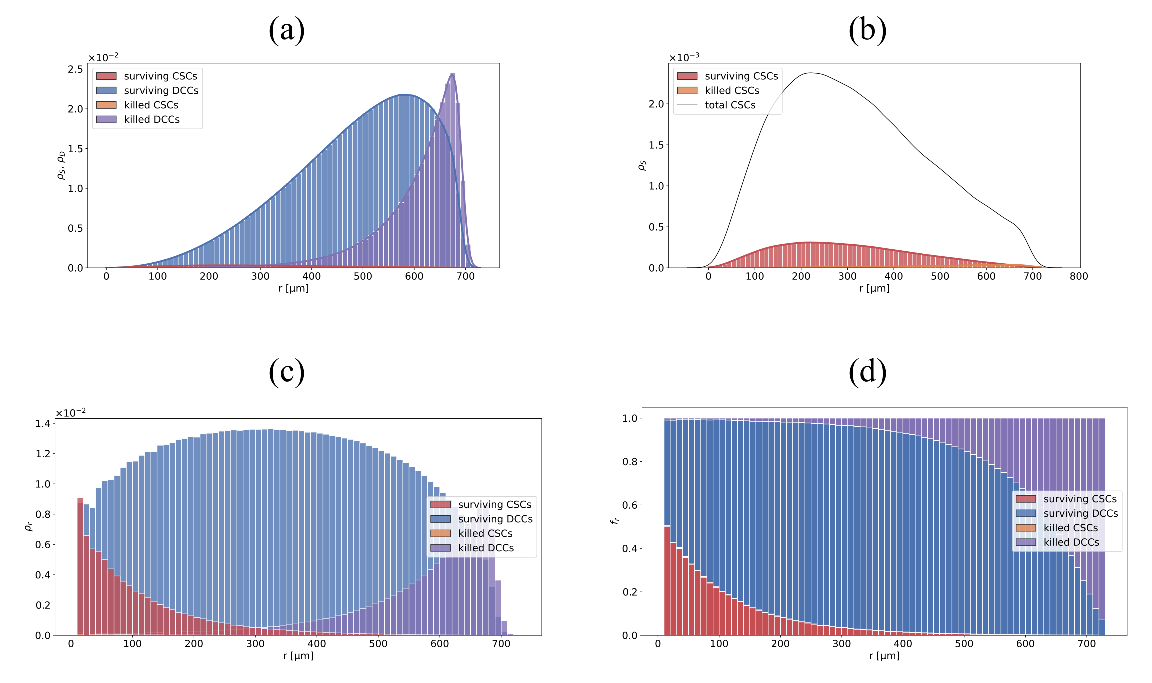
\includegraphics[width=1.0\linewidth]{./images/S1.eps}
	\caption{\emph{Cell distributions for 60-day-old tumorspheres after therapy.}  (a) Killed and surviving CSC and DCC distributions display the same shape as those for 30-day old tumorspheres. The CSC population is too small to be clearly visible and is rescaled in the next panel. (b) Expanded view of the surviving and killed CSC distributions. (c) Radial dependence of the cell density shows CSCs are mainly located far from the surface. (d) Cell fraction profiles reveal that cells would be protected within the core of the tumorsphere.  No killed CSCs are detectable at this scale.}
	\label{fig:S1}
\end{figure}

\begin{figure}[ht]
	\centering
	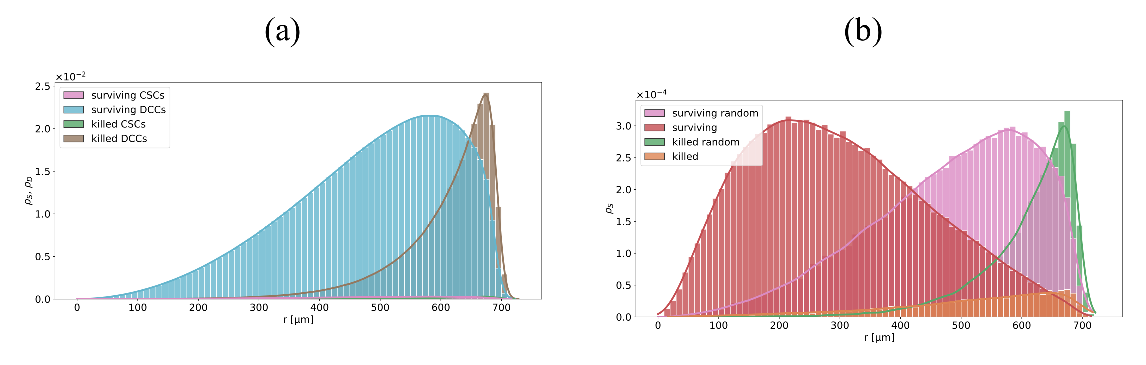
\includegraphics[width=1.0\linewidth]{./images/S2.eps}
	\caption{\emph{Effect of radiotherapy on a 60-day-old tumorsphere with a random CSC distribution.} Histograms show cell numbers as a function of distance from the tumorsphere center. (a) CSC and DCC spatial distributions display the same overall shape, although their total numbers differ greatly. [En esta escala las CSC no se ven; se podrian poner en la misma grafica los numeros de CSC multiplicados por 10, por ejemplo] (b) Comparison between the CSC distributions in our model (cf. Fig S1b) with those resulting from a random cell allocation shows that the CSC survival is higher in our model.}
	\label{fig:S2}
\end{figure}

\begin{figure}[ht]
	\centering
	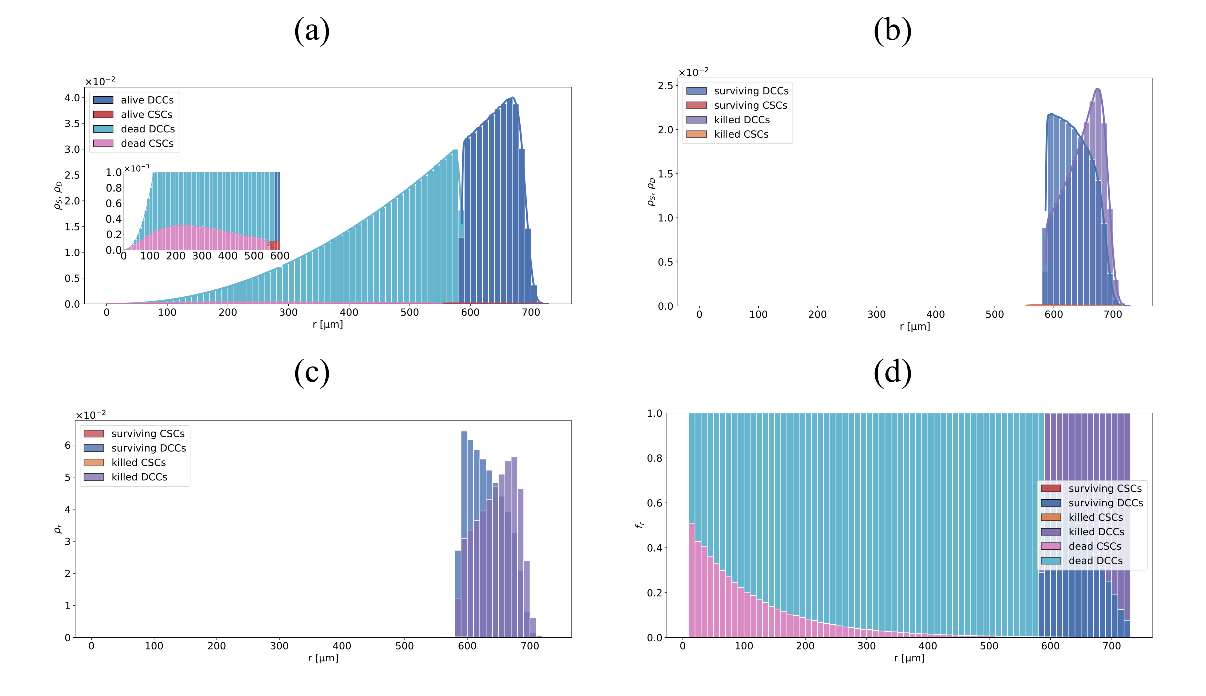
\includegraphics[width=1.0\linewidth]{./images/S3.eps}
	\caption{\emph{Combined effects of hypoxia and radiation on 60-day tumorspheres} reveals a complete absence oflive CSCs for $c_S=0.23$ and $c_D=0.30$. This is a consequence of our assumption that CSC cannot survive at very low $O_2$ concentrations. (a) Before the therapy, the tumorsphere has developed a necrotic core of radius $ R_N = 590 \mu m$. The inset highlights the hypoxic CSC range showing a very small fraction of live CSCs located far from the center due to the stringent threshold.  (b) Cell distribution after a single dose of radiotherapy; for clarity, cells that were already dead at the time of the therapy are not shown. All surviving CSCs were killed by therapy. (c) Histograms from (b) rescaled to show the radial dependence of the cell concentrations. (d) Cell fraction profiles for all cell types highlighting the CSC annihilation resulting from  the strict anoxic threshold $c_S$.}
	\label{fig:S3}
\end{figure}



%\section*{Supplementary References}
%\addcontentsline{toc}{section}{Supplementary References}
% If SI has its own references, put them here. With BibTeX, easiest is a second .bib or same .bib with only SI citations.
% \bibliographystyle{unsrt}
% \bibliography{biblio}

% ========== END OF SUPPLEMENTARY MATERIALS ===========











\end{document}
\endinput
%%
%% End of file `elsarticle-template-num.tex'.
